\documentclass[a4paper,11pt]{article}

\title{M\'etodos Num\'ericos en E.D.P. II}
\author{Jos\'e Angel de Bustos P\'erez}

\usepackage[spanish]{babel}
\usepackage{graphicx}
\addtolength{\voffset}{-3cm}

\hyphenation{e-qui-va-len-tes}

\begin{document}

\maketitle
\thispagestyle{empty}
\newpage

\section{Problema continuo}

El problema que vamos a resolver es el siguiente:

\begin{displaymath}
-\gamma \ \Delta \ \Psi = 0 \qquad en \ \Omega
\end{displaymath}
donde $\gamma = 1$, entonces como el segundo miembro de la igualdad es cero
se tiene que:

\begin{displaymath}
\Delta \ \Psi = \frac{\partial \Psi}{\partial x^2}+
\frac{\partial \Psi}{\partial y^2} = 0 \qquad en \ \Omega
\end{displaymath}

\subsection{Problema a resolver}

Como sabemos que las lineas de corriente se definen $\Psi (x,y) =$ cte, que el
caudal de corriente que circula entre dos lineas se define como $\Psi_1-\Psi_2$
y que la velocidad aguas arriba es de $5\ cm/s$ entonces el caudal que circula a
trav\'es de la secci\'on ser\'a de $5 \times 4=20\ cm^2/s$, luego podemos
suponer que:\newline \newline

\setlength{\unitlength}{3947sp}%
%
\begingroup\makeatletter\ifx\SetFigFont\undefined%
\gdef\SetFigFont#1#2#3#4#5{%
  \reset@font\fontsize{#1}{#2pt}%
  \fontfamily{#3}\fontseries{#4}\fontshape{#5}%
  \selectfont}%
\fi\endgroup%
\begin{picture}(7224,3060)(1189,-3136)
\thinlines
\put(1201,-361){\line( 0,-1){2400}}
\put(1201,-2761){\line( 1, 0){7200}}
\put(8401,-2761){\line( 0, 1){1050}}
\put(8401,-1711){\line(-1, 0){2300}}%2400
\put(6101,-1711){\line(-5, 3){2250.294}}%2360.294
\put(3841,-361){\line(-1, 0){2640}}%2400
\put(2701,-211){\makebox(0,0)[lb]{\smash{\SetFigFont{12}{14.4}{\rmdefault}{\mddefault}{\updefault}$\Psi_F = 20$ $cm^2/s$}}}
\put(2701,-3136){\makebox(0,0)[lb]{\smash{\SetFigFont{12}{14.4}{\rmdefault}{\mddefault}{\updefault}$\Psi_I = 0$ $cm^2/s$}}}
\end{picture}

\ \\
Observemos que en las lineas verticales que definen el dominio se tiene que:

\begin{displaymath}
\sum_{i=1}^2 \frac{\partial \Psi}{\partial x_i}\cdot \gamma_i = 0 \qquad sobre \ 
\Gamma
\end{displaymath}
donde $x_1= x$, $x_2=y$ y $\gamma_i$ es la componente i$-$esima de la normal.

\newpage

Luego el problema a resolver ser\'a:\\

Hallar $\Psi \in H^1(\Omega )$ tal que:

\begin{displaymath}
\Delta \ \Psi = 0\qquad en \ \Omega \\
\end{displaymath}
verificando las siguientes condiciones de contorno:
\begin{displaymath}
\Psi_I = 0 \qquad \Psi_F = 20
\end{displaymath}
\begin{displaymath}
\sum_{i=1}^2 \frac{\partial \Psi}{\partial x_i}\cdot \gamma_i = 0\qquad sobre \ 
\Gamma
\end{displaymath}
donde

\begin{displaymath}
H^1(\Omega )=\{ f \in L^2(\Omega )\ |\qquad \frac{\partial f}{\partial x_i}
\in L^2(\Omega )\ i=1,2 \}
\end{displaymath}

\section{Formulaci\'on variacional}

Multipliquemos por $v\in H^1(\Omega )$, entonces se tiene:

\begin{displaymath}
\Delta \ \Psi \cdot v = 0\qquad \forall \ v \in H^1(\Omega )
\end{displaymath}
integrando en $\Omega $ tenemos que:

\begin{displaymath}
\int_{\Omega }\Delta \ \Psi \cdot v = 0 \qquad \forall \ v \in H^1(\Omega )
\end{displaymath}
aplicando ahora la f\'ormula de Green tenemos que:

\begin{displaymath}
-\sum_{i=1}^2 \int_{\Omega } \frac{\partial \Psi}{\partial x_i}\cdot
\frac{\partial v}{\partial x_i}+\sum_{i=1}^2\int_{\Gamma }
\frac{\partial \Psi }{\partial x_i}\cdot \gamma_i \cdot v = 0\qquad \forall \
v \in H^1(\Omega )
\end{displaymath}
teniendo en cuenta la linealidad de la integral y las condiciones de contorno,
tenemos que:

\begin{displaymath}
\sum_{i=1}^2\int_{\Gamma }\frac{\partial \Psi}{\partial x_i}\cdot \gamma_i
\cdot v = \int_{\Gamma} \sum_{i=1}^2 \frac{\partial \Psi}{\partial x_i}\cdot
\gamma_i \cdot v = 0\qquad \forall \ v \in H^1(\Omega )
\end{displaymath}
Luego la formulaci\'on variacional del problema ser\'a la siguiente:\\

Hallar $u\in H^1(\Omega )$ tal que:

\begin{displaymath}
\sum_{i=1}^2 \int_{\Omega } \frac{\partial \Psi}{\partial x_i}\cdot
\frac{\partial v}{\partial x_i} = 0\qquad \forall \ v \in H^1(\Omega )
\end{displaymath}

\newpage

\subsection{Notaciones}

En lo sucesivo utilizaremos las siguientes notaciones:

\begin{displaymath}
a\ (\Psi , v) = \sum_{i=1}^2 \int_{\Omega }\frac{\partial \Psi}{\partial x_i}
\cdot \frac{\partial \Psi}{\partial x_i}
\end{displaymath}

\begin{displaymath}
L\ (v) = 0\qquad \forall \ v \in H^1(\Omega )
\end{displaymath}

\subsection{Existencia y soluci\'on del problema variacional}

Para ello utilizaremos el teorema de \emph{Lax$-$Milgram}, para ello se tiene
que verificar que:

\begin{itemize}
\item $L\ (\cdot )$ sea lineal y continuo.
\item $a\ (\cdot ,\cdot)$ sea bilineal, continuo y el\'{\i}ptico.
\end{itemize}
Como $L\ (\cdot )$ es la funci\'on nula entonces es claro que es lineal y
continua.\\ \\
Que $a\ (\cdot ,\cdot )$ sea bilineal es inmediato pues la integral es lineal.\\
\\
Para la continuidad de $a\ (\cdot ,\cdot )$ utilizaremos lo siguiente:

\begin{displaymath}
|v|^2_{1,\Omega } = \sum_{i=1}^2 \int_{\Omega } \ ( \ 
\frac{\partial v}{\partial x_i}\ )^2\qquad \forall \ v \in H^1(\Omega )
\end{displaymath}

\begin{displaymath}
||v||^2_{1,\Omega }= \int_{\Omega }v^2\ + \sum_{i=1}^2 \int_{\Omega } \ ( \
\frac{\partial v}{\partial x_i}\ )^2\qquad \forall \ v \in H^1(\Omega )
\end{displaymath}
Entonces tendremos lo siguiente:

\begin{equation} \label{eq:semiequivalencia}
||v||^2_{\Omega } = \int_{\Omega }v^2\ + \sum_{i=1}^2 \int_{\Omega }\ ( \
\frac{\partial v}{\partial x_i}\ )^2 \ge \sum_{i=1}^2 \int_{\Omega }\ ( \
\frac{\partial v}{\partial x_i}\ )^2 = |v|^2_{1,\Omega }
\end{equation}

\newpage

Veamos la continuidad de $a\ (\cdot ,\cdot )$.\\ \\
Utilizando la definici\'on de $a\ (\cdot ,\cdot )$ y utilizando
``Cauchy$-$Schwarz'' tenemos que:

\begin{displaymath}
|a\ (\Psi ,v)| = |\sum_{i=1}^2 \int_{\Omega }\frac{\partial \Psi}{\partial x_i}
\frac{\partial v}{\partial x_i}| \le \sqrt{\sum_{i=1}^2 \int_{\Omega }
(\frac{\partial \Psi}{\partial x_i})^2 }\cdot \sqrt{\sum_{i=1}^2\int_{\Omega }
(\frac{\partial v}{\partial x_i})^2} = |\Psi |_{1,\Omega }\cdot |v|_{1,\Omega }
\end{displaymath}
utilizando $(\ref{eq:semiequivalencia})$ se tiene que:

\begin{displaymath}
|a\ (\Psi ,v)| \le |\Psi |_{1,\Omega }\cdot |v|_{1,\Omega } \le
||\Psi ||_{1,\Omega }\cdot ||v||_{1,\Omega }
\end{displaymath}
y dado que $a\ (\cdot ,\cdot )$ es bilineal entonces es continua.\\ 

Veamos ahora la el\'{\i}pticidad de $a\ (\cdot ,\cdot)$.\\ \\
Para que $a\ (\cdot ,\cdot )$  sea el\'{\i}ptica se tiene que verificar que
exista una constante $\alpha > 0$ verificando:

\begin{equation} \label{eq:elipticidad}
a\ (v,v) \ge \alpha \cdot ||v||^2_{1,\Omega }\qquad \forall \ v \in H^1(\Omega )
\end{equation}
Por definici\'on de $a\ (\cdot ,\cdot )$ se tiene que:

\begin{displaymath}
a\ (v,v) = \sum_{i=1}^2 \int_{\Omega } (\frac{\partial v}{\partial x_i})^2 =
|v|^2_{1,\Omega }\qquad \forall \ v \in H^1(\Omega )
\end{displaymath}
Si la seminorma $|\cdot |_{1,\Omega}$ fuera equivalente a la norma
$||\cdot ||_{1,\Omega }$ entonces se verificar\'{\i}a $(\ref{eq:elipticidad})$,
y $a\ (\cdot ,\cdot )$ ser\'{\i}a el\'{\i}ptica.\\ \\
En $H^1_0 (\Omega )$ ambas son equivalentes, pero en $H^1 (\Omega )$ no lo
son\footnote{O al menos no he sido capaz de demostrarlo.}. Por lo tanto
supondremos que existe un subespacio de $H^1(\Omega )$, tambi\'en de Hilbert,
en el cual ambas son equivalentes.\\ \\
Suponiendo esto entonces $a\ (\cdot , \cdot )$ ser\'{\i}a el\'{\i}ptica y
estar\'{\i}amos en las condiciones del teorema de \emph{Lax$-$Milgram}, con lo
cual el problema variacional tendr\'{\i}a soluci\'on \'unica y todo lo hecho
hasta aqu\'{\i} ser\'{\i}a valido con cambiar todas las referencias a
$H^1(\Omega )$ por dicho subespacio.

\newpage

El problema que he encontrado, y por el cual he supuesto la existencia de un
subespacio de Hilbert en el cual la seminorma y la norma sean equivalentes, es
el comportamiento de la soluci\'on sobre la frontera, ya que los casos
estudiados en clase o bien la soluci\'on se anulaba en la frontera o era igual
a una funci\'on de $H^{1/2}(\Gamma )$ (y utilizabamos el teorema de la traza) o
bien teniamos una condici\'on de tipo Newman en la frontera.

\subsection{Equivalencia con el problema de partida}

$\Rightarrow |$ Si $\Psi $ verifica el problema continuo es claro que $\Psi $
verifica la formulaci\'on d\'ebil del problema.\\ \\
$\Leftarrow |$ Si $\Psi $ verifica la formulaci\'on d\'ebil en particular
verifica:

\begin{displaymath}
\sum_{i=1}^2 \int_{\Omega } \frac{\partial \Psi}{\partial x_i}
\frac{\partial v}{\partial x_i} = 0\qquad \forall \ v \in \mathcal{D}(\Omega )
\end{displaymath}
es decir:

\begin{displaymath}
\sum_{i=1}^2 <\frac{\partial \Psi}{\partial x_i},
\frac{\partial v}{\partial x_i}> = 0\qquad \forall \ v \in \mathcal{D}(\Omega )
\end{displaymath}

\begin{displaymath}
<\Delta \ \Psi,v> = 0\qquad \forall \ v \in \mathcal{D}(\Omega )
\end{displaymath}
es decir recuperamos la ecuaci\'on de partida, pero en el sentido de las
distribuciones.

\newpage

\section{Resoluci\'on pr\'actica}

Para resolver el problema hemos utilizado el programa \emph{ANSYS} y los
resultados obtenidos han sido los siguientes.

\subsection{Elementos}

Los elementos utilizados fueron cuadrados con cuatro nodos.\\

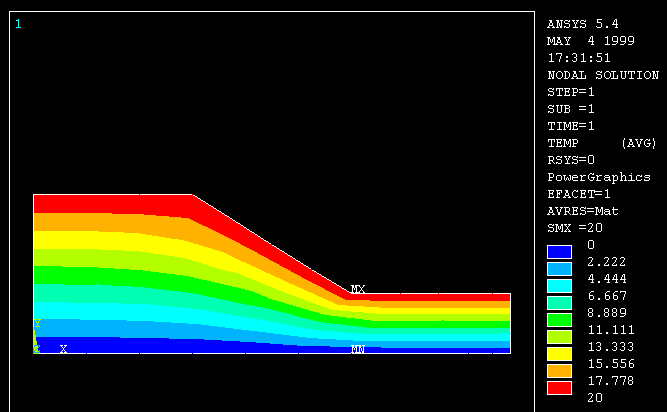
\includegraphics[scale=0.5]{4nodos.png}

\newpage

\subsection{Mallado}

Una vez construido el recinto, el cual no tiene simetrias que pudieramos
utilizar para simplificar el modelo, y generado el mallado correspondiente, en 
el cual habi\'{\i}a elementos grandes procedimos a refinarlo. \\

El mallado que utilizamos para resolver el problema fue el siguiente:\\

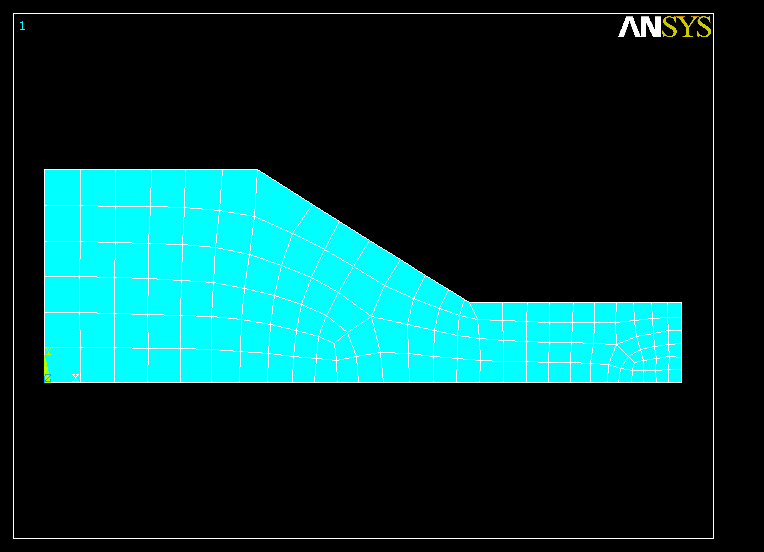
\includegraphics[scale=0.5]{malla2.png}

\newpage

\subsection{Soluci\'on}

La soluci\'on del problema es la siguiente:\\

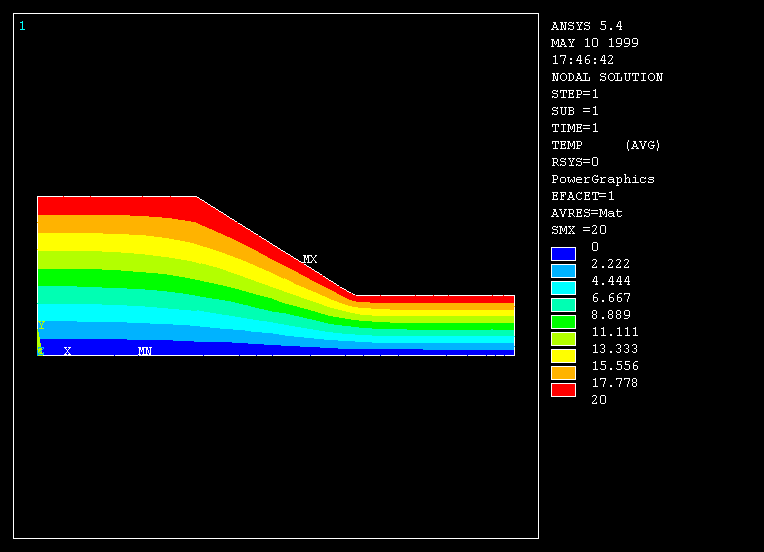
\includegraphics[scale=0.5]{solucion.png}

\end{document}
